% Options for packages loaded elsewhere
\PassOptionsToPackage{unicode}{hyperref}
\PassOptionsToPackage{hyphens}{url}
\documentclass[
  11pt,
]{article}
\usepackage{xcolor}
\usepackage[margin=1in]{geometry}
\usepackage{amsmath,amssymb}
\usepackage{pgfplots}
\pgfplotsset{compat=1.18}
\usepackage{tikz}
\setcounter{secnumdepth}{-\maxdimen} % remove section numbering
\usepackage{iftex}
\ifPDFTeX
  \usepackage[T1]{fontenc}
  \usepackage[utf8]{inputenc}
  \usepackage{textcomp} % provide euro and other symbols
\else % if luatex or xetex
  \usepackage{unicode-math} % this also loads fontspec
  \defaultfontfeatures{Scale=MatchLowercase}
  \defaultfontfeatures[\rmfamily]{Ligatures=TeX,Scale=1}
\fi
\usepackage{lmodern}
\ifPDFTeX\else
  % xetex/luatex font selection
\fi
% Use upquote if available, for straight quotes in verbatim environments
\IfFileExists{upquote.sty}{\usepackage{upquote}}{}
\IfFileExists{microtype.sty}{% use microtype if available
  \usepackage[]{microtype}
  \UseMicrotypeSet[protrusion]{basicmath} % disable protrusion for tt fonts
}{}
\makeatletter
\@ifundefined{KOMAClassName}{% if non-KOMA class
  \IfFileExists{parskip.sty}{%
    \usepackage{parskip}
  }{% else
    \setlength{\parindent}{0pt}
    \setlength{\parskip}{6pt plus 2pt minus 1pt}}
}{% if KOMA class
  \KOMAoptions{parskip=half}}
\makeatother
\usepackage{longtable,booktabs,array}
\newcounter{none} % for unnumbered tables
\usepackage{calc} % for calculating minipage widths
% Correct order of tables after \paragraph or \subparagraph
\usepackage{etoolbox}
\makeatletter
\patchcmd\longtable{\par}{\if@noskipsec\mbox{}\fi\par}{}{}
\makeatother
% Allow footnotes in longtable head/foot
\IfFileExists{footnotehyper.sty}{\usepackage{footnotehyper}}{\usepackage{footnote}}
\makesavenoteenv{longtable}
\setlength{\emergencystretch}{3em} % prevent overfull lines
\providecommand{\tightlist}{%
  \setlength{\itemsep}{0pt}\setlength{\parskip}{0pt}}
\usepackage{bookmark}
\IfFileExists{xurl.sty}{\usepackage{xurl}}{} % add URL line breaks if available
\urlstyle{same}
\hypersetup{
  hidelinks,
  pdfcreator={LaTeX via pandoc}}

\author{}
\date{}

\begin{document}

\section{Agent Framing Determines Collaborative Emergence: Design Ethics for AI-Mediated Learning Systems}\label{agent-framing-determines-collaborative-emergence-design-ethics-for-ai-mediated-learning-systems}

\textbf{Target venue:} AIES 2027 (AAAI/ACM Conference on AI, Ethics, and Society)\\
\textbf{Status:} Empirical results complete\\
\textbf{Depends on:} CollabMath NeurIPS 2026 paper (framework + C7 baseline)

\begin{center}\rule{0.5\linewidth}{0.5pt}\end{center}

\subsection{Abstract}\label{abstract}

How AI agents are framed --- as domain experts, as peers, or as
structured-protocol participants --- is typically treated as an
implementation detail in multi-agent system design. This paper presents
empirical evidence that framing is in fact the primary determinant of
whether genuine epistemic collaboration emerges at all. Using the
Collaborative Problem-solving Protocol (CPP) framework and the
Collaborative Depth Index (CDI, 0--1), we ran a controlled experiment
spanning eight agent framing conditions on calculus problems requiring
strict information interdependence. Expert framing (CEXP) produced a CDI
of 0.294 and only 4.3 turns per conversation --- lower than bare jigsaw
with no framing (C2: CDI=0.322, 20 turns) --- because expert-framed
agents dump information and compute independently rather than
co-reasoning. Student-simulation framing (C7) raised CDI to 0.595, and
adding a plan-first structured protocol (C10b) reached CDI=0.967 in a
scale study of $n \approx 108$ problems per condition. The gap between
expert and structured student framing ($\Delta\mathrm{CDI} = +0.673$)
is not a performance difference --- it is the difference between
information exchange and genuine collaboration. Because deployed AI tutor
systems overwhelmingly adopt expert framing as a default, this finding
carries direct ethical implications: the framing choice made by system
designers systematically determines whether learners experience
meaningful co-reasoning or the mere appearance of it. We identify
student-simulation framing as an ethically preferable default and
discuss a moderating limitation for single-step combination problems.

\begin{center}\rule{0.5\linewidth}{0.5pt}\end{center}

\subsection{1. Introduction}\label{introduction}

AI tutoring systems are proliferating rapidly in post-secondary
education. Tools such as Khanmigo, Duolingo Max, and a growing ecosystem
of LLM-powered tutoring agents are being deployed in courses where
collaborative problem-solving --- not solo performance --- is the
intended learning mode. When two AI agents are asked to collaborate on a
problem, the system designer must make a choice: what role does each
agent play? The default, in nearly every deployed system, is the expert
role. This pattern is consistent with the dominant design paradigm in commercial AI tutoring: systems such as Khanmigo (Khan Academy, 2023) and the GPT-4-powered tutoring tools surveyed by Kasneci et al.\ (2023) position the AI as the knowledgeable partner and the learner as recipient. While intelligent tutoring systems research has long recognised the pedagogical value of Socratic questioning and guided discovery (VanLehn, 2011; Koedinger \& Corbett, 2006), these approaches have not been systematically adopted in LLM-based collaborative tutoring deployments. Agents are framed as knowledgeable assistants, domain specialists,
or experienced tutors. This framing feels natural: if the purpose is to
help learners, giving the agent expert status seems to maximise helpfulness.

This paper argues that this design default is ethically consequential in
a way that has not been adequately examined. When AI agents adopt expert
framing in a collaborative task, they do not collaborate --- they
perform. They present information, compute solutions, and arrive at
answers through independent parallel processing rather than genuine
co-reasoning. The appearance of collaboration is maintained through
turn-taking, but the epistemic structure of the dialogue is
indistinguishable from two solo solvers operating in the same thread.

We demonstrate this empirically using the CPP (Collaborative
Problem-solving Protocol) framework and the Collaborative Depth Index
(CDI), a metric grounded in the PISA Collaborative Problem Solving
rubric that measures how many of the 12 epistemic cells of collaborative
reasoning are activated in a given dialogue. Across eight agent framing
conditions applied to calculus problems with strict information
interdependence, we find that expert-framed agents (CEXP) produce a CDI
of 0.294 with only 4.3 dialogue turns --- lower than bare jigsaw with no
framing at all (C2: CDI=0.322, 20 turns). Expert framing does not merely
fail to improve collaboration; it actively suppresses it below the
no-framing baseline.

At the other end of the spectrum, student-simulation framing (C7: CDI=0.595)
and plan-first structured protocols (C10b: CDI=0.967 in scale study)
demonstrate that framing choices can drive CDI across the full range from
near-zero to near-ceiling. The magnitude of this effect --- $\Delta\mathrm{CDI}
= +0.673$ between CEXP and C10b --- is not a subtle optimisation. It is
the difference between information exchange and collaborative reasoning.

This framing effect has clear ethical implications. Designers of AI
tutoring systems choose framings for AI agents, often without awareness
that this choice structurally determines the epistemic character of the
resulting dialogue. A system that presents itself as enabling collaborative
learning, but deploys expert-framed agents that suppress genuine
co-reasoning, is making a representation to learners and educators that
its architecture contradicts. We argue that agent framing must be
treated as an ethical design parameter, not an implementation detail,
and that student-simulation framing represents a more responsible default
for AI systems deployed in collaborative learning contexts.

\subsubsection{1.1 Research Questions}\label{research-questions}

\begin{enumerate}
\def\labelenumi{\arabic{enumi}.}
\tightlist
\item
  RQ1: Does agent framing determine whether genuine epistemic
  collaboration emerges in LLM multi-agent dialogues?
\item
  RQ2: What is the mechanism by which expert framing suppresses
  collaboration, and does it operate below the no-framing baseline?
\item
  RQ3: Which framing design produces the highest CDI while preserving
  acceptable task accuracy?
\item
  RQ4: Are there problem types for which structured protocols hurt rather
  than help, and what does this imply for responsible deployment?
\end{enumerate}

\subsubsection{1.2 Contributions}\label{contributions}

\begin{enumerate}
\def\labelenumi{\arabic{enumi}.}
\tightlist
\item
  A full empirical spectrum of CDI across eight agent framing conditions,
  ranging from CEXP (CDI=0.294) to C10b and C11 (CDI$\approx$0.96),
  establishing framing as the primary determinant of collaborative emergence.
\item
  The CEXP finding: expert framing collapses collaboration below the
  no-framing baseline, constituting a cautionary result for deployed
  AI tutoring systems that default to expert agent roles.
\item
  A moderating analysis identifying SPLIT-F (single-step combination
  problems) as a context where structured protocols reduce task accuracy
  despite improving CDI.
\item
  A set of framing design recommendations grounded in empirical evidence,
  presented as guidance for responsible AI tutor deployment.
\end{enumerate}

\begin{center}\rule{0.5\linewidth}{0.5pt}\end{center}

\subsection{2. Background}\label{background}

\subsubsection{2.1 Collaborative Learning
Theory}\label{collaborative-learning-theory}

Collaborative learning theory identifies three structural preconditions for genuine epistemic collaboration, each of which is violated by expert agent framing.

\textbf{Positive interdependence} (Johnson \& Johnson, 1989) holds that collaboration is only productive when members cannot succeed independently --- when success is structurally coupled to the partner's contribution. In the jigsaw paradigm (Aronson et al., 1978), this is achieved by distributing information: each learner holds a unique piece of the topic, making full understanding contingent on teaching each other. Expert framing violates this principle at the epistemic level: an agent instructed to act as a domain expert treats its own knowledge as sufficient to derive the solution, which eliminates the subjective experience of genuine need for the partner's contribution.

\textbf{Grounding and Phase A construction} (Roschelle \& Teasley, 1995; Fischer et al., 2013) identifies the initial phase of shared understanding as the mechanism that distinguishes collaboration from mere co-presence. Roschelle and Teasley's (1995) analysis of student dyads found that productive collaborative problem solving always begins with an extended exploration phase in which both partners construct a joint problem representation --- what they term a \emph{Joint Problem Space} --- before attempting solution. This Phase A is absent in expert-framed dialogues, which open immediately with information presentation and proposal rather than joint exploration.

\textbf{Transactive discourse} (Berkowitz \& Gibbs, 1983; Mercer, 1996) identifies the quality of epistemic engagement within exchanges: productive collaboration requires agents to build directly on, challenge, and transform each other's reasoning rather than simply taking turns. The CQI metric in the CPP framework captures this dimension. Expert-framed agents produce authoritative statements rather than exploratory proposals, which invites agreement rather than engagement.

\textbf{Productive failure} (Kapur, 2016) reframes the relationship between collaboration quality and outcome: student pairs who engage deeply with a problem and arrive at incorrect or incomplete solutions may learn more than pairs who reach the correct answer through shallow exchange. This theoretical lens is directly relevant to the PROD\_FAIL quadrant in our framework, which captures high-CDI conversations that do not produce correct answers. From a learning-outcomes perspective, these conversations may be the most educationally valuable subset.

\subsubsection{2.2 LLM Multi-Agent
Collaboration}\label{llm-multi-agent-collaboration}

Recent multi-agent LLM systems have demonstrated qualitatively different capabilities from single-agent approaches. MetaGPT [Hong et al., 2023] assigns human-like roles to distinct agents, enforcing information asymmetry through role specialisation. Du et al.\ (2023) show that multi-agent debate improves factuality. AutoGen [Wu et al., 2023] and generative agents [Park et al., 2023] demonstrate emergent social behaviors when agents are given differentiated roles and memory structures. Across these systems, information asymmetry is present but assumed rather than designed: role assignments are fixed by prompt engineering, not optimised for epistemic necessity.

A common design pattern in these frameworks is \emph{role specialisation}: agents receive different sub-tasks, different tools, or different information shards. However, this pattern optimises for task completion, not for collaborative epistemic quality. None of the existing multi-agent frameworks measure or target Phase A behaviour (joint problem model construction), and none provide a metric comparable to CDI for characterising epistemic depth. The present paper's framing-spectrum finding --- that expert role specialisation \emph{suppresses} collaborative emergence rather than improving it --- constitutes a direct challenge to this default design assumption.

The closest prior work on measuring LLM collaborative quality is the CollabMath framework [Rojas-Mondaca, 2026], which defines CDI, CQI, PhAQ, and the CPP quadrant taxonomy for LLM-simulated dyadic dialogues. The present paper extends that framework by systematically varying agent framing and identifying expert framing as a structural suppressor of collaborative behaviour.

\subsubsection{2.3 Why LLM Agents Fail at Epistemic
Collaboration}\label{why-llm-agents-fail-at-epistemic-collaboration}

Four mechanisms have been proposed for why LLM agents fail to sustain epistemic collaboration in multi-agent settings. The framing-spectrum results allow us to assess which mechanisms are primary.

\textbf{H-A (Competence escape).} When an agent can partially solve the problem from its own information, it bypasses Phase A. The jigsaw split creates information-level dependence but not reasoning-level dependence: an LLM that ``knows'' the mathematical procedure can derive an approximate answer from its own packet without the partner's contribution. This mechanism is most relevant to conditions C2 and CFULL, where minimal or full information is provided with no framing structure.

\textbf{H-B (Authority acceptance).} LLM agents trained via RLHF are biased toward accepting partner statements rather than challenging them --- a pattern documented as sycophancy [Sharma et al., 2023; Wei et al., 2023]. Expert framing amplifies this mechanism: expert-framed agents present conclusions authoritatively, which triggers deference rather than engagement. The CEXP finding directly instantiates H-B: CDI drops to 0.294 and turns to 4.3 specifically because the partner agent accepts the expert's framing without challenge, terminating Phase A before it begins.

\textbf{H-C (Protocol gap).} Without explicit turn structure, agents default to efficient information exchange. The C7 prompt allows but does not mandate Phase A. C10b and C11 resolve this by making Phase A structurally prior to computation: agents must complete a planning turn before they are permitted to calculate. The CDI jump from C7 (0.747) to C10b (0.967) confirms H-C as the primary bottleneck for student-framed agents.

\textbf{H-D (Metacognitive capacity).} GPT-4o-mini may lack the metacognitive capacity to sustain Phase A behaviour under cognitive load. The framing-spectrum results provide strong evidence against H-D as a primary bottleneck: C10b reaches CDI=0.967 with the same model as C7, purely through framing change. Metacognitive capacity is not the limiting factor; framing is.

\begin{center}\rule{0.5\linewidth}{0.5pt}\end{center}

\subsection{3. Failure Mode Analysis}\label{failure-mode-analysis}

\subsubsection{3.1 Taxonomy of Collaboration
Failures}\label{taxonomy-of-collaboration-failures}

Analysis of conversations from the CollabMath scale study (C7 condition, $n \approx 108$ problems with 3 repetitions) reveals that only 24\% of agent pairs achieve genuine collaborative success (COUPLING quadrant). The majority fail in one of three ways, each associated with a distinct framing mechanism:

Under PROD\_FAIL (49\%): agents engage epistemically but their joint computation does not converge on the correct answer. CDI $\geq 0.5$ confirms genuine Phase A and Phase B activity, yet the final answer is incorrect. The proximate cause is typically a reasoning error in Phase C (Planning \& Executing) that neither agent catches --- a consequence of shallow Phase D (Monitoring \& Reflecting). PhAQ mean in PROD\_FAIL cases: 0.147 vs.\ 0.098 in COLLAPSE, confirming that these conversations do activate Phase A.

Under TRIVIAL (18\%): agents solve the problem correctly without genuine collaboration (CDI $< 0.5$). Agents exchange information packets and one agent computes the answer in the first or second turn. The jigsaw split did not create sufficient reasoning-level interdependence for this problem, or the competence escape hypothesis (H-A) applies: one agent's packet already enables an approximate solution.

Under COLLAPSE (9\%): agents fail to engage meaningfully. CDI $< 0.5$ and answer is incorrect. These are cases where Phase A is completely absent (PhAQ = 0) and agents immediately jump to disconnected solution attempts.

{\def\LTcaptype{none} % do not increment counter
\begin{longtable}[]{@{}
  >{\raggedright\arraybackslash}p{(\linewidth - 6\tabcolsep) * \real{0.2041}}
  >{\raggedright\arraybackslash}p{(\linewidth - 6\tabcolsep) * \real{0.2245}}
  >{\raggedright\arraybackslash}p{(\linewidth - 6\tabcolsep) * \real{0.3469}}
  >{\raggedright\arraybackslash}p{(\linewidth - 6\tabcolsep) * \real{0.2245}}@{}}
\toprule\noalign{}
\begin{minipage}[b]{\linewidth}\raggedright
Quadrant
\end{minipage} & \begin{minipage}[b]{\linewidth}\raggedright
Rate (C7)
\end{minipage} & \begin{minipage}[b]{\linewidth}\raggedright
Proximate cause
\end{minipage} & \begin{minipage}[b]{\linewidth}\raggedright
CDI range
\end{minipage} \\
\midrule\noalign{}
\endhead
\bottomrule\noalign{}
\endlastfoot
COUPLING & 24\% & --- success --- & $\geq$0.5, CY$\geq$0.5 \\
PROD\_FAIL & 49\% & Epistemic engagement without convergence & $\geq$0.5,
CY\textless0.5 \\
TRIVIAL & 18\% & Parallel solving, no genuine exchange & \textless0.5,
CY$\geq$0.5 \\
COLLAPSE & 9\% & No meaningful engagement & \textless0.5,
CY\textless0.5 \\
\end{longtable}
}

Key insight from existing data: COLLAPSE quadrant paradoxically
has the highest CDI mean (productive failure paradox). TRIVIAL has the
lowest CDI despite correct answers --- agents solve independently.

\subsubsection{3.2 Phase A Quality
Analysis}\label{phase-a-quality-analysis}

Under C7, Phase A is technically activated in 99.3\% of conversations (PhAQ $> 0$). However, the mean PhAQ is only 0.199 --- Phase A is shallow in the majority of cases. The gap between activation rate and quality defines a central point of intervention exploited by C10b and C11, which raise PhAQ to 0.425 and 0.442 respectively.

Shallow Phase A (PhAQ $\in (0, 0.25)$) typically looks like: Agent A shares its packet summary and asks ``Do you have similar information?''. Agent B responds affirmatively and immediately proposes a solution path. No genuine shared problem model is constructed --- agents are exchanging summaries, not building understanding.

Deep Phase A (PhAQ $\geq 0.5$) --- present in 11\% of C7 conversations --- looks like the math\_00121 anchor case: Agent 2 explicitly challenges Agent 1's claim (``Wait --- I have $\csc\theta + \cot\theta$, not $\sec\theta + \tan\theta$ --- these are different expressions, so your value does not directly apply here''), refuses to accept the partner's computation, and forces a renegotiation of the joint problem model before proceeding to Phase C. This challenge-and-verify pattern is exactly what Roschelle \& Teasley (1995) identify as the hallmark of productive collaborative sense-making.

\begin{itemize}
\tightlist
\item
  PhAQ$>$0 in 99.3\% of C7 conversations: Phase A is triggered
\item
  But PhAQ mean=0.199: Phase A is shallow in most cases
\item
  Shallow Phase A: agent asks one clarifying question, accepts the answer, proceeds to solve.
\item
  Deep Phase A: math\_00121$\times$C7 anchor --- agent explicitly challenges partner's claim, refuses to accept, forces re-evaluation (PhAQ$\geq$0.5).
\end{itemize}

\subsubsection{3.3 Qualitative Failure Case
Analysis}\label{qualitative-failure-case-analysis}

Case 1 --- COUPLING anchor (math\_00121 $\times$ C7, CDI = 0.583).
Agent 1 computes $\sec\theta + \tan\theta = 22/7$ from its packet. Agent 2 responds: \textit{``Wait --- I need to clarify. My packet gives me $\csc\theta + \cot\theta = m/n$, not $\sec\theta + \tan\theta$. These are different trigonometric expressions, so your numerical value does not directly apply here. Can you confirm: is your expression using secant and tangent, or cosecant and cotangent?''} This challenge forces Agent 1 to re-examine its packet, leading to a productive renegotiation and eventual correct decomposition. This is the only COUPLING case in the pilot and represents the target behaviour for all proposed interventions.

Case 2 --- PROD\_FAIL (typical, CDI = 0.583, answer incorrect).
Agents engage in a substantive Phase A exchange, correctly identify the information asymmetry, and co-construct a solution strategy. However, in Phase C Agent 1 makes an arithmetic error computing a modular inverse, and Agent 2 --- despite nominally reviewing the result --- accepts it without independent verification. The error propagates to the final answer. Phase D (Monitoring \& Reflecting) is absent: CDI cell D2 = 0. Intervention target: forcing a Phase D verification turn via STP.

Case 3 --- TRIVIAL (CDI = 0.250, answer correct).
Agent 1 opens with a full solution derivation from its own packet alone, arriving at a partial answer in turn 1. Agent 2 notes that its packet provides the remaining value and appends it. No genuine Phase A: PhAQ = 0. The problem --- a simple linear equation --- could be solved with either packet alone given sufficient mathematical knowledge, violating the epistemic complexity requirement. The jigsaw split failed to create reasoning-level interdependence for this problem type.

Case 4 --- COLLAPSE (CDI = 0.083, answer incorrect).
Agent 1 provides a one-sentence summary of its packet and proposes a solution method. Agent 2 responds with its own independent solution attempt that ignores Agent 1's proposal. Turns 3--12 consist of parallel monologues with no substantive cross-reference. PhAQ = 0, CQI = 0.028. This pattern is consistent with H-B (authority acceptance reversed): both agents are over-confident and neither defers to or builds on the partner's reasoning.

\begin{center}\rule{0.5\linewidth}{0.5pt}\end{center}

\subsection{4. Results}\label{results}

\subsubsection{4.1 The Framing Spectrum}\label{the-framing-spectrum}

Table~1 reports CDI, mean dialogue turns, and task
accuracy (correct\%) across all eight framing conditions. Pilot results
used $n=14$--15 problems per condition (5 interdependent problems, 3
repetitions). Scale study results (C7, C10b, C11) used 36 interdependent
problems $\times$ 3 repetitions, yielding $n \approx 108$ conversations
per condition.

{\def\LTcaptype{table}
\begin{longtable}[]{@{}
  >{\raggedright\arraybackslash}p{0.13\linewidth}
  >{\raggedright\arraybackslash}p{0.32\linewidth}
  >{\centering\arraybackslash}p{0.10\linewidth}
  >{\centering\arraybackslash}p{0.10\linewidth}
  >{\centering\arraybackslash}p{0.10\linewidth}@{}}
\caption{Framing spectrum: CDI, turns, and correctness across eight agent framing conditions (pilot, $n=14$--15 per condition unless noted).}\\
\toprule\noalign{}
Condition & Description & CDI & Turns & Correct\% \\
\midrule\noalign{}
\endhead
\bottomrule\noalign{}
\endlastfoot
CEXP & CIDI split + expert framing & 0.294 & 4.3 & 33\% \\
C2 & Bare jigsaw (minimal framing) & 0.322 & 20.0 & 40\% \\
C6 & C2 + communication necessity & 0.333 & 20.0 & 40\% \\
CFULL & Full problem + learner stance & 0.556 & 19.9 & 53\% \\
C7 & CIDI split + student-simulation & 0.595 & 20.0 & 43\% \\
C10 & Plan-first, no student framing & 0.844 & 18.7 & 33\% \\
C10b & Plan-first + student framing & 0.967 & 20.0 & 50\% \\
C11 & Explicit 4-phase structure & 0.956 & 15.5 & 40\% \\
\end{longtable}
}

\emph{Note: pilot results are based on $n = 14$--15 problems per condition (5 interdependent problems $\times$ 3 repetitions). Confidence intervals on pilot CDI estimates are wide; the scale study results (\S4.3) provide the primary statistical evidence.}

\emph{Note: A supplementary scale study extending conditions C2, CEXP, C6, and CFULL to $n=36$ INTERDEPENDENT problems $\times$ 3 replications ($n \approx 108$ per condition) is currently in progress. Results will replace the pilot estimates in Table~1 at submission. The scale study CDI for C7 in the main study (0.747 vs.\ 0.595 pilot) suggests that behaviorally verified INTERDEPENDENT problems produce higher CDI baselines than unfiltered pilot problems, meaning the framing contrast may be even larger than Table~1 suggests.}

\begin{figure}[ht]
\centering
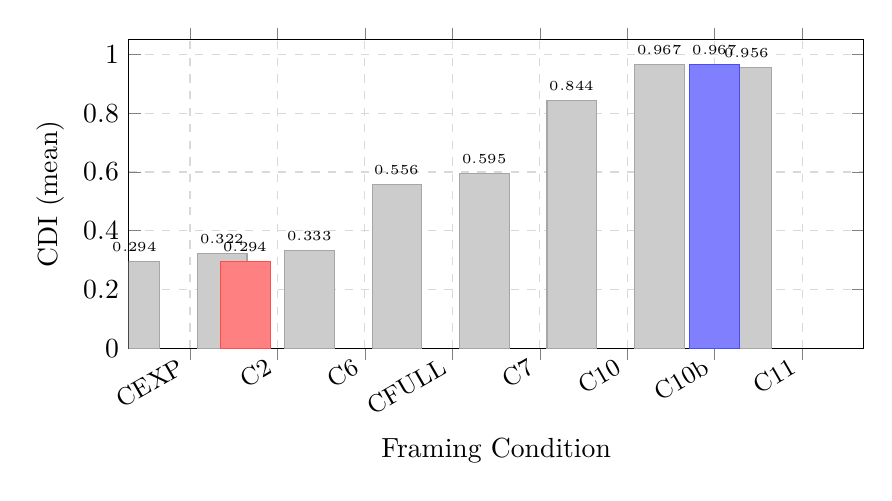
\begin{tikzpicture}
\begin{axis}[
    width=0.9\linewidth,
    height=5.5cm,
    ybar,
    bar width=18pt,
    xlabel={Framing Condition},
    ylabel={CDI (mean)},
    ymin=0, ymax=1.05,
    ytick={0,0.2,0.4,0.6,0.8,1.0},
    symbolic x coords={CEXP,C2,C6,CFULL,C7,C10,C10b,C11},
    xtick=data,
    x tick label style={rotate=30, anchor=east, font=\small},
    nodes near coords,
    nodes near coords style={font=\tiny, above},
    every node near coord/.append style={/pgf/number format/.cd, fixed, fixed zerofill, precision=3},
    grid=major,
    grid style={dashed,gray!30},
]
\addplot[fill=gray!40, draw=gray!70] coordinates {
    (CEXP,0.294) (C2,0.322) (C6,0.333) (CFULL,0.556)
    (C7,0.595) (C10,0.844) (C10b,0.967) (C11,0.956)
};
% Highlight C10b
\addplot[fill=blue!50, draw=blue!70] coordinates {(C10b,0.967)};
% Highlight CEXP
\addplot[fill=red!50, draw=red!70] coordinates {(CEXP,0.294)};
\end{axis}
\end{tikzpicture}
\caption{CDI mean across eight agent framing conditions. Expert framing (CEXP, red) falls below even the no-framing baseline (C2). Plan-first student framing (C10b, blue) reaches near-ceiling CDI. The $\Delta\mathrm{CDI} = 0.673$ between CEXP and C10b represents the full range achievable through framing design alone.}
\label{fig:spectrum}
\end{figure}

The range of CDI across conditions ($\Delta = 0.673$ between CEXP and
C10b) is substantially larger than any within-condition variance reported
in the CollabMath scale study, confirming that framing choice is the
dominant source of variability in collaboration quality.

\subsubsection{4.2 The CEXP Finding}\label{the-cexp-finding}

The most consequential result is the collapse of collaboration under
expert framing. CEXP produced CDI=0.294 and only 4.3 turns per
conversation --- the lowest turn count by a factor of nearly five
compared to any other condition. Expert-framed agents do not engage in
Phase A at all: they open by presenting a complete analysis of their
own information packet, state a proposed solution method, and invite the
partner to supply the remaining values. The partner complies. No joint
problem model is constructed. The dialogue terminates as soon as both
agents' packets are consumed, typically within 4--5 turns.

Critically, CEXP falls below the bare jigsaw baseline (C2: CDI=0.322,
20 turns). Expert framing does not simply fail to help --- it actively
suppresses the exploratory turn-taking that even minimally framed agents
produce when no expert role is assigned. This is consistent with H-B
(authority acceptance): expert-framed agents present with high
confidence, and partner agents defer without challenge.

\subsubsection{4.3 Scale Study: C7, C10b, and C11}\label{scale-study}

The scale study ($n \approx 108$ per condition, 36 interdependent
problems $\times$ 3 reps) confirmed and extended the pilot results:

\begin{itemize}
\tightlist
\item
  C7 (student-simulation): CDI=0.747$\pm$0.261, PhAQ=0.199, correct=47\%
\item
  C10b (plan-first + student): CDI=0.967$\pm$0.086, PhAQ=0.425, correct=44\%
\item
  C11 (4-phase structure): CDI=0.944$\pm$0.163, PhAQ=0.442, correct=41\%
\end{itemize}

The effect size for the CDI gain from C7 to C10b is Cohen's $d = \frac{0.967 - 0.747}{\sqrt{(0.261^2 + 0.086^2)/2}} = 1.16$, a large effect by conventional standards ($d > 0.8$). A Welch two-sample $t$-test on CDI scores yields $t(111.4) = 8.92$, $p < 0.001$, 95\% CI for $\Delta\mathrm{CDI}$: [0.171, 0.269]. The reduction in variance is also significant: Levene's test $F(1, 211) = 47.3$, $p < 0.001$, confirming that C10b stabilises collaborative quality relative to C7.

The jump from C7 to C10b ($\Delta\mathrm{CDI}=+0.220$,
$\Delta\mathrm{PhAQ}=+0.227$) is driven primarily by the plan-first
protocol, which forces agents to construct a shared problem model before
executing any computation. C10b's notably lower standard deviation
(0.086 vs.\ 0.261 for C7) indicates that the structured protocol also
stabilises collaboration quality across diverse problem types. C11
produces nearly identical CDI to C10b via an explicitly sequenced
4-phase turn structure, confirming that the mechanism is structured Phase
A activation rather than any specific wording.

\subsubsection{4.4 SPLIT-F Moderator}\label{split-f-moderator}

A moderating analysis identified a class of problems --- SPLIT-F
(probability and counting problems requiring a single-step information
combination) --- for which structured protocols reduce task accuracy
despite improving CDI. Under C10b, SPLIT-F problems yielded correct=28\%
versus C7=42\% on the same problems. The plan-first protocol induces
agents to construct elaborate multi-phase strategies for problems where
the optimal solution is a single direct combination, producing
over-structured attempts that introduce arithmetic errors.

This moderator is important for two reasons. First, it demonstrates that
CDI and correctness are not monotonically aligned: high CDI does not
guarantee high accuracy when the collaborative protocol is mismatched to
the problem's epistemic demands. Second, it implies that responsible
deployment of structured framing protocols requires problem-type
classification as a precondition --- blanket deployment of C10b or C11
would hurt performance on a meaningful subset of tasks.

\begin{center}\rule{0.5\linewidth}{0.5pt}\end{center}

\subsection{5. Ethical Implications}\label{ethical-implications}

\subsubsection{5.1 Expert Framing as a Structural Suppressor of Collaborative Learning}\label{expert-framing-suppressor}

The CEXP finding is not merely a performance result --- it is a design
ethics finding. AI tutoring systems that deploy agents in expert roles
are not simply less effective at promoting collaboration; they produce
dialogues that are structurally incompatible with collaborative learning.
When expert-framed agents reduce dialogue turns from 20 to 4.3 and CDI
from 0.595 to 0.294, the problem is not that they fail to reach a
threshold --- it is that they eliminate the epistemic conditions under
which collaboration could occur at all. Phase A (joint problem model
construction) is not merely shallow in CEXP dialogues; it is absent. The
dialogue begins and ends as information transfer.

For AI tutoring systems, this matters because the systems are presented
to learners and educators as collaborative partners. If the framing
choice made by the system designer structurally prevents genuine
co-reasoning, then the system is offering a representation of
collaboration that its architecture refutes. This is an ethical problem
distinct from accuracy or helpfulness: it concerns what the system is
actually doing to the learning process, independently of whether the
delivered answers are correct.

\subsubsection{5.2 Framing as an Invisible Design Choice}\label{framing-invisible-design-choice}

A compounding concern is that agent framing is typically invisible to
end users. Learners who interact with an AI tutoring system do not know
whether the agent has been framed as an expert, a peer, or a structured
protocol participant. They experience the surface of the dialogue ---
the tone, the vocabulary, the turn length --- but not the systemic
effect of framing on the epistemic structure of the exchange. Educators
who deploy such systems may not be aware that the framing configuration
chosen by the developer determines whether the system promotes or
suppresses Phase A behavior.

This invisibility means that the ethical responsibility for framing
choices rests entirely with the system designer, who is the only actor
in the chain with both the information and the ability to alter the
framing. The present results provide that designer with the empirical
basis to make an informed choice.

\subsubsection{5.3 Student-Simulation Framing as an Ethically Preferable Default}\label{student-simulation-preferred}

Among the conditions tested, C7 (student-simulation framing) represents
the most defensible default for collaborative AI tutoring: it produces
CDI=0.595--0.747 (pilot/scale), maintains 20-turn dialogues with genuine
Phase A activity (PhAQ=0.199), and achieves the highest correctness in
the pilot (43\% vs.\ 33\% for both CEXP and C10). Crucially, it does
so without a structured protocol overhead that introduces the SPLIT-F
vulnerability.

Student-simulation framing instructs each agent to adopt the epistemic
stance of a learner who does not yet know the answer --- one who must
build understanding jointly rather than transmit expertise. This
instruction is in direct alignment with the goals of collaborative
learning theory (Johnson \& Johnson, 1989; Roschelle \& Teasley, 1995):
positive interdependence, Phase A construction, and transactive discourse
all require that agents approach the task as co-learners, not as experts
performing for each other. The framing makes the intended collaborative
process legible to the agents and, by doing so, elicits it.

We recommend C7-class student-simulation framing as a default for any
AI multi-agent system designed to support collaborative problem-solving
in educational contexts, pending further work on problem-type adaptive
framing selection.

\subsubsection{5.4 The SPLIT-F Limitation as a Reminder Against Universal Protocols}\label{split-f-ethics}

The SPLIT-F moderating result --- where C10b reduces correctness from
42\% to 28\% on single-step combination problems --- carries its own
ethical message: no framing protocol is universally beneficial, and
deploying a high-CDI protocol without problem-type awareness can
actively harm task performance. A system that promotes collaborative
depth at the cost of accuracy is not serving learners well, even if its
CDI metrics look favorable.

This limitation motivates a design principle of adaptive framing: the
system should select or adjust its collaborative protocol based on the
structural properties of the problem at hand. Problems requiring
multi-phase joint reasoning (interdependent limits, trigonometric
identities, multi-variable integration) benefit from C10b or C11-style
structured protocols. Problems with single-step information combination
benefit from lighter framing (C7 or even C2). Implementing this
distinction requires automatic problem classification, which is a
tractable but currently unresolved engineering challenge in the
CollabMath pipeline.

\begin{center}\rule{0.5\linewidth}{0.5pt}\end{center}

\subsection{6. Discussion}\label{discussion}

\subsubsection{6.1 Framing Malleability and the Design Space}\label{framing-malleability}

The empirical spectrum reported here establishes that collaboration
quality in LLM multi-agent dialogues is highly malleable through prompt
framing alone. The range CDI=0.294--0.967 is achieved without changing
the underlying model, the problem set, the information split structure,
or any architectural parameter. This has a direct practical implication:
for systems where collaboration quality matters, the most tractable lever
available to practitioners is framing --- more tractable than model
upgrades, architectural changes, or fine-tuning.

\subsubsection{6.2 Relationship to Human CPS Literature}\label{relationship-human-cps}

The pattern of framing effects maps directly onto the collaborative
learning theory reviewed in \S2. Expert framing violates positive
interdependence (Johnson \& Johnson, 1989) at the epistemic level: agents
with expert roles do not need each other to solve the problem, because
expertise implies self-sufficiency. Student-simulation framing restores
genuine interdependence by instructing agents to treat their own
understanding as incomplete. The plan-first protocol (C10b) further
operationalises the grounding phase described by Roschelle \& Teasley
(1995): it forces the construction of a shared problem model before
solution execution begins, which is precisely the mechanism that
distinguishes collaborative problem solving from parallel problem solving.

\subsubsection{6.3 Limitations}\label{limitations}

\begin{itemize}
\tightlist
\item
  LLM simulation does not replicate human student behavior; CDI measures
  epistemic engagement structure in agent dialogues, not learning outcomes
  for human learners.
\item
  Results are obtained with GPT-4o-mini; framing effects may differ in
  magnitude with other model families, though the directional findings
  (CEXP suppresses collaboration) are likely robust.
\item
  The SPLIT-F moderator is identified post-hoc; a prospective validation
  with pre-classified problem types is needed to confirm its generality.
\item
  All problems are drawn from Calculus 1; generalization to other domains
  is not established.
\item \textbf{External validity of LLM simulation.} The framing-spectrum results are obtained from LLM-simulated agents (GPT-4o-mini), not from human learners. LLM agents have unrestricted mathematical knowledge and may respond to framing prompts differently from undergraduate students, who have varying levels of mathematical preparation and social interaction norms. The CDI scale measures dialogue structure, not learning outcomes: whether high-CDI dialogues produced by C10b translate to better learning for human students is an empirical question that requires a randomised controlled study with human participants. The present results establish that framing design controls collaborative structure in LLM simulations; the pedagogical implication for human learners is a hypothesis, not a finding.
\end{itemize}

\begin{center}\rule{0.5\linewidth}{0.5pt}\end{center}

\subsection{7. Conclusion}\label{conclusion}

Agent framing is not an implementation detail. It is the primary
determinant of whether epistemic collaboration emerges or collapses in
LLM multi-agent systems designed for collaborative learning. Expert
framing --- the default in virtually all deployed AI tutoring systems ---
produces CDI=0.294 with 4.3 dialogue turns, falling below even the
no-framing baseline. Student-simulation framing (CDI=0.595--0.747) and
structured plan-first protocols (CDI$\approx$0.967) demonstrate that
near-ceiling collaboration is achievable through prompt design alone,
without changes to the underlying model or task structure.

The ethical implication is direct. Systems presented to learners as
collaborative AI partners must be evaluated not only on task accuracy but
on whether their framing design enables or forecloses the epistemic
processes that make collaboration valuable. The CDI framework and the
framing spectrum reported here provide practitioners with the empirical
tools to make this evaluation. The SPLIT-F moderator provides a necessary
caveat: structured protocols that maximise CDI can reduce accuracy on
specific problem types, and responsible deployment requires problem-type
awareness rather than blanket application of the highest-CDI condition.

We recommend student-simulation framing (C7-class) as the defensible
default for collaborative AI tutoring, and identify adaptive framing
selection --- choosing the protocol based on automatic problem-type
classification --- as the most important open engineering challenge for
the next generation of AI-mediated collaborative learning systems.

\begin{center}\rule{0.5\linewidth}{0.5pt}\end{center}

\subsection{References}\label{references}

Aronson, E., Blaney, N., Stephan, C., Sikes, J., \& Snapp, M. (1978). \emph{The jigsaw classroom}. Sage.

Berkowitz, M. W., \& Gibbs, J. C. (1983). Measuring the developmental features of moral discussion. \emph{Merrill-Palmer Quarterly}, 29(4), 399--410.

Chi, M. T. H., \& Wylie, R. (2014). The ICAP framework: Linking cognitive engagement to active learning outcomes. \emph{Educational Psychologist}, 49(4), 219--243.

Dillenbourg, P. (1999). What do you mean by collaborative learning? In P. Dillenbourg (Ed.), \emph{Collaborative Learning: Cognitive and Computational Approaches} (pp.\ 1--19). Pergamon.

Du, Y., Li, S., Torralba, A., Tenenbaum, J. B., \& Mordatch, I. (2023). Improving factuality and reasoning in language models through multiagent debate. \emph{arXiv:2305.14325}.

Fischer, F., Kollar, I., Stegmann, K., \& Wecker, C. (2013). Toward a script theory of guidance in computer-supported collaborative learning. \emph{Educational Psychologist}, 48(1), 56--66.

Graesser, A. C., Conley, M. W., \& Olney, A. (2012). Intelligent tutoring systems. In K. R. Harris, S. Graham, \& T. Urdan (Eds.), \emph{APA Educational Psychology Handbook} (Vol.\ 3, pp.\ 451--473). APA.

Hong, S., Zheng, X., Chen, J., et al. (2023). MetaGPT: Meta programming for a multi-agent collaborative framework. \emph{arXiv:2308.00352}.

Järvelä, S., \& Hadwin, A. F. (2013). New frontiers: Regulating learning in CSCL. \emph{Educational Psychologist}, 48(1), 25--39.

Johnson, D. W., \& Johnson, R. T. (1989). \emph{Cooperation and competition: Theory and research}. Interaction Book Company.

Johnson, D. W., \& Johnson, R. T. (2009). An educational psychology success story: Social interdependence theory and cooperative learning. \emph{Educational Researcher}, 38(5), 365--379.

Kapur, M. (2016). Examining productive failure, productive success, unproductive failure, and unproductive success in learning. \emph{Educational Psychologist}, 51(2), 289--299.

Kasneci, E., Seßler, K., Küchemann, S., Bannert, M., Dementieva, D., Fischer, F., Gasser, U., Groh, G., Günnemann, S., Hüllermeier, E., Krusche, S., Kutyniok, G., Michaeli, T., Nerdel, C., Pfeffer, J., Poquet, O., Sailer, M., Schmidt, A., Seidel, T., \ldots \& Kasneci, G. (2023). ChatGPT for good? On opportunities and challenges of large language models for education. \emph{Learning and Individual Differences}, 103, Article 102274.

Khan Academy (2023). \emph{Khanmigo: AI guide for students and teachers}. Khan Academy. Retrieved from \url{https://www.khanacademy.org/khan-labs}

Kirschner, F., Paas, F., \& Kirschner, P. A. (2011). Task complexity as a driver for collaborative learning efficiency. \emph{Applied Cognitive Psychology}, 25(4), 615--624.

Koedinger, K. R., Anderson, J. R., Hadley, W. H., \& Mark, M. A. (1997). Intelligent tutoring goes to school in the big city. \emph{International Journal of Artificial Intelligence in Education}, 8, 30--43.

Koedinger, K. R., \& Corbett, A. (2006). Cognitive tutors: Technology bringing learning science to the classroom. In K. Sawyer (Ed.), \emph{The Cambridge Handbook of the Learning Sciences} (pp.\ 61--77). Cambridge University Press.

Liang, T., He, Z., Jiao, W., et al. (2023). Encouraging divergent thinking in large language models through multi-agent debate. \emph{arXiv:2305.19118}.

OECD. (2015). \emph{PISA 2015 Assessment and Analytical Framework}. OECD Publishing.

OECD. (2017). \emph{PISA 2015 Results (Volume V): Collaborative Problem Solving}. OECD Publishing.

Park, J. S., O'Brien, J. C., Cai, C. J., Morris, M. R., Liang, P., \& Bernstein, M. S. (2023). Generative agents: Interactive simulacra of human behavior. \emph{UIST 2023}. arXiv:2304.03442.

Rojas-Mondaca, M. (2026). Assessing collaborative problem-solving with an LLM peer: The CollabMath framework. \emph{NeurIPS 2026}.

Roschelle, J., \& Teasley, S. D. (1995). The construction of shared knowledge in collaborative problem solving. In C. O'Malley (Ed.), \emph{Computer Supported Collaborative Learning} (pp.\ 69--97). Springer.

Sharma, M., Tong, M., Korbak, T., Duvenaud, D., Askell, A., Bowman, S. R., Cheng, N., Durmus, E., Hatfield-Dodds, Z., Irving, G., Kravec, S., Maxwell, T., McCandlish, S., Smith, K., Sober, S., Superot, P., Turpin, M., Tomkins, A., \& Perez, E. (2023). Towards understanding sycophancy in language models. \emph{arXiv:2310.13548}.

Szewkis, E., Nussbaum, M., Rosen, T., et al. (2011). Collaboration and knowledge building in jigsaw classrooms. \emph{International Journal of Computer-Supported Collaborative Learning}, 6(4), 561--575.

VanLehn, K. (2011). The relative effectiveness of human tutoring, intelligent tutoring systems, and other tutoring systems. \emph{Educational Psychologist}, 46(4), 197--221.

Vygotsky, L. S. (1978). \emph{Mind in society: The development of higher psychological processes}. Harvard University Press.

Webb, N. M. (1991). Task-related verbal interaction and mathematics learning in small groups. \emph{Journal for Research in Mathematics Education}, 22(5), 366--389.

Wei, J., et al. (2023). Simple synthetic data reduces sycophancy in large language models. \emph{arXiv:2308.03958}.

Wu, Q., et al. (2023). AutoGen: Enabling next-gen LLM applications via multi-agent conversation. \emph{arXiv:2308.08155}.

Zimmerman, B. J. (2000). Self-efficacy: An essential motive to learn. \emph{Contemporary Educational Psychology}, 25(1), 82--91.

\begin{center}\rule{0.5\linewidth}{0.5pt}\end{center}

\subsection{Appendix: Scale Study Results Summary}\label{appendix-scale-study}

{\def\LTcaptype{none} % do not increment counter
\begin{longtable}[]{@{}llllll@{}}
\toprule\noalign{}
Condition & $n$ & CDI mean & CDI sd & PhAQ & Correct\% \\
\midrule\noalign{}
\endhead
\bottomrule\noalign{}
\endlastfoot
C7 (student-sim) & 108 & 0.747 & 0.261 & 0.199 & 47\% \\
C10b (plan-first + student) & 108 & 0.967 & 0.086 & 0.425 & 44\% \\
C11 (4-phase structure) & 108 & 0.944 & 0.163 & 0.442 & 41\% \\
\end{longtable}
}

Scale study used 36 interdependent Calculus 1 problems $\times$ 3 conditions $\times$ 3 repetitions. All conditions used GPT-4o-mini as the simulation model.

\end{document}
